\documentclass[twocol]{ametsocV6.1}
\usepackage{hyperref}
\usepackage[separate-uncertainty=true]{siunitx}
\usepackage{csvsimple}
\usepackage{ifthen}
\usepackage{cprotect}
\usepackage{comment}
\usepackage{tabularx}
\usepackage{makecell}

\DeclareSIUnit\clight{\text{\ensuremath{c}}}
\renewcommand{\sectionautorefname}{\S}
\renewcommand{\subsectionautorefname}{\S}
\renewcommand{\subsubsectionautorefname}{\S}

\let\subsectionautorefname\sectionautorefname

\title{
	Experimental assessment of the capabilities and limitations of
	NaI(Tl) scintillation-based gamma ray spectrometry
}

\authors{
	Thomas Schanzer \aff{a}
	\correspondingauthor{
		Thomas Schanzer,\\ t.schanzer@student.unsw.edu.au \\
		\emph{Word count:} 3696 words
	}
}

\affiliation{\aff{a}{
	School of Physics, University of New South Wales,
	Sydney, Australia
}}

\abstract{
	We present measurements of the gamma ray spectra of six radioisotopes
	using a thallium-doped sodium iodide scintillation detector.
	We first explain the appearances of the spectra and calibrate the
	detector to allow energy measurements. We then analyse the spectra
	to derive three key measures of detector performance: resolution,
	intrinsic width and full energy peak efficiency. We relate the values of
	these parameters and their dependence on gamma ray energy to the
	capabilities and fundamental limitations of scintillation detection.
}

\begin{document}
\maketitle

\section{Introduction}\label{sec:intro}
The decay of unstable nuclei may result in the release of excess energy
in the form of high-energy photons known as gamma rays, created when the
product nuclei transition from excited to lower-energy states. The gamma ray
energies produced by a given radionuclide are precisely determined by
the energies of the initial and final states and therefore take on a discrete
spectrum that is unique to the radionuclide \citep[p. 191]{lannunziata_2006}.

The uniqueness of the spectra makes gamma spectrometry an invaluable tool
in many applications that require the analysis of radioactive samples of
unknown isotopic composition. \cite{mero_1960}, for example, demonstrates
that it may be used to determine the uranium or thorium content of natural
ores in the mining industry. The \emph{Lunar Prospector} orbiter,
launched in 1998, carried a gamma ray spectrometer that it used to map the
distribution of radionuclides on the Moon's surface in an effort to
``improve our understanding of lunar formation and evolution''
\citep{lawrence_et_al_1998}.

\subsection{Gamma ray detection}
We have noted that the spectrum of gamma rays emitted by a radionuclide is
discrete.
In order to detect the gamma rays and measure their energies, however,
they must be made to interact with and deposit energy in matter.
We will show that observed spectra therefore differ from emitted spectra; the
interaction mechanisms must be understood in order to interpret them.

The first interaction mechanism in gamma ray detectors is Compton scattering,
whereby a photon is deflected by a stationary electron.
It may be shown that the kinetic energy imparted to an electron
(mass $m_e$) by a photon
of energy $E$, undergoing Compton scattering at an angle $\theta$, is
\[\displaystyle
    E \frac{
        2 \left(E/\left(m_e c^2\right)\right) \sin^2 (\theta/2)
    }{
        1 + 2 \left(E/\left(m_e c^2\right)\right) \sin^2 (\theta/2)
    }.
\]
The angle dependence of the energy thus deposited into the detector material
produces a continuous distribution of energies in the measured spectrum,
known as the \emph{Compton continuum}.
The continuum has a finite extent, terminating at the \emph{Compton edge}
\begin{equation}
	E_c = \frac{2E^2}{m_e c^2 + 2E},
	\label{eqn:compton_edge}
\end{equation}
where $\theta = \pi$ (i.e., when the photon is scattered back along its
direction of incidence)
and the maximum possible energy is deposited into the
detector.

The second interaction mechanism is the photoelectric effect, which involves
the absorption of a gamma photon's energy by an electron, ejecting it from
its host atom. The electron then comes to rest in the detector material,
such that the entire photon energy is deposited. The photoelectric effect is
dominant at low energies ($\lesssim \SI{2e2}{\kilo\electronvolt}$ for
the detector used in this work) but diminishes rapidly with increasing
energy, leaving Compton scattering as the dominant process at higher energies
\citep{notes}.

Measurement of the deposited energy may be achieved by using a crystal
doped with a \emph{phosphor}, whose atoms radiate part of the deposited
energy as light, as the detector material. The minute amounts of light
emitted by the crystal (the \emph{scintillator}) are then amplified
by a photomultiplier tube. Incoming photons eject photoelectrons
from a cathode, which are accelerated between a series of electrodes
(\emph{dynodes}) of increasing electric potential.
At each dynode, each incoming electron ejects multiple secondary electrons,
producing a charge cascade and an easily measurable voltage pulse 
at the final anode \citep[p. 13]{hamamatsu_2007}. Key to the energy measurement
is the fact that the amplitude of the pulse is proportional to the
energy deposited in the scintillator; this allows the instrument to be
calibrated.

\begin{figure}[ht]
	\centering
	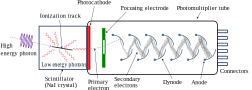
\includegraphics[width=\linewidth]{../figures/detection_diagram.pdf}
	\caption{
		Diagram of the scintillator and photomultiplier tube used to 
		detect gamma photons.
		Adapted from \cite{detector_diagram} under the
		Creative Commons Attribution-Share Alike 3.0 Unported license.
	}
\end{figure}

\subsection{Typical gamma ray spectra}
The aforementioned interactions of the gamma photons with the detector,
along with other interactions in the surrounding shielding
\citep{crosthwaite_2022} complicate
the interpretation of the resulting spectra. A monochromatic source will
not produce a single sharp peak, but rather a wider \emph{full energy peak}
or \emph{photopeak}
corresponding to photons whose entire energy is deposited in the detector
and a lower-energy Compton continuum corresponding to incomplete energy
transfer via Compton scattering.

Of particular interest is the width (FWHM), $\Delta E$, of the full energy peak,
which determines the resolving power of the spectrometer (i.e., its ability to
distinguish two closely-spaced energies). If the cascading arrival of
electrons at the anode of the photomultiplier tube is modelled as a Poisson
process, with each arrival independent of the last, the amplitude of a
voltage pulse (and the measured gamma ray energy) should have a standard
deviation proportional to the square root of the average amplitude:
$\Delta E \propto \sqrt{E}$. Basic manipulations then yield
$(\Delta E/E)^2 = B/E$ for some constant $B$. In real detectors, however,
the arrivals are not entirely independent, leading to the empirical expression
\begin{equation}
	\left( \frac{\Delta E}{E} \right)^2 = \frac{B}{E} + W_I^2,
	\label{eqn:resolution}
\end{equation}
where the constant $W_I$ is known as the \emph{intrinsic width} of the
detector \citep{notes}. Observe that the resolution $\Delta E/E$ improves
with increasing energy. In the limit as $E \to \infty$, $W_I$ is the
best resolution that may be achieved.

\subsection{Overview}
In \autoref{sec:methods}, we will describe the configuration and operation
of the particular spectrometer used in this work and our approach to
characterising the peaks in our spectra. \autoref{sec:results} will
present the results of our measurements and their analysis, beginning
by explaining the appearances of the spectra and then considering the
calibration, resolution and full energy peak efficiency of the detector.
\autoref{sec:discussion} will discuss the two primary limitations and sources
of uncertainty in our experiment and propose solutions for implementation
in future work.

\section{Methods} \label{sec:methods}
The scintillator used in this work was a thallium-doped sodium iodide
(NaI(Tl)) crystal, contained in a lead housing into which the radioisotope
samples were lowered. The photomultiplier pulses were amplified, then
digitised by a multi-channel analyser, allowing them to be sorted into
2048 amplitude bins of equal width, ideally corresponding to 2048 energy bins
of equal width.

Six radioisotopes were tested: $^{241}$Am, $^{133}$Ba, $^{60}$Co, $^{137}$Cs,
$^{152}$Eu and $^{22}$Na. For each radioisotope sample, counting was conducted
for a known period of time and the resulting number of pulses in each of the
2048 bins was recorded. For a full description of the measurement setup
and the instruments used, refer to the student notes \citep{notes}.

The count data were analysed and visualised using Python 3.9. Two methods
for extracting the locations and widths of peaks were used and evaluated.
The first involved fitting a Lorentzian function of the form
\begin{equation}
	y =\frac{a}{1 + \left( \frac{x - x_0}{\mathrm{FWHM}/2} \right)^2} + b
	\label{lorentzian}
\end{equation}
to the part of the spectrum in the immediate vicinity of each peak
using ordinary least-squares regression.
The uncertainty in the number of pulses, $n$, falling in a given
amplitude bin was estimated by $\sqrt{n}$ in accordance with Poisson
statistics (gamma ray arrivals are random, independent and steady over time),
and this was passed as an argument to the fitting function.
We thus obtained the height $a$, base $b$, location $x_0$ and FWHM of each peak.

The alternative was to use the pre-made peak finding routine
$\verb|scipy.signal.find_peaks|$ in SciPy 1.7.3 \citep{scipy}. The routine
takes the channel with the highest count as the centre of the peak;
to reduce the influence of noise on this determination, the spectra were
smoothed using a Gaussian filter with standard deviation $\sigma = 2$.
It then draws a horizontal line through the top of each peak,
using the points on the left and right where the line intersects
the spectrum again (or else the endpoints of the dataset) to delineate
a basin on each side of the peak. The higher of the lowest points in the left
and right basins is taken to be the baseline.
The width is then measured halfway between the baseline and maximum of the peak.

The advantages and disadvantages of the two methods are discussed in
\autoref{sec:discussion}, but since their results differed in places and
neither gave entirely satisfactory results, the final values for the peak
parameters were found by averaging the outputs of the Lorentzian fit and
the $\verb|find_peaks|$ routine (with Gaussian pre-smoothing of the spectra).
The locations of the maxima prior to Gaussian smoothing were also included.
The uncertainties were taken
to be half the range of these values, with a minimum uncertainty of one
channel imposed to eliminate unrealistic values.

\section{Results} \label{sec:results}
\begin{figure*}[p]
	\vspace{-0.8cm}
	\centerline{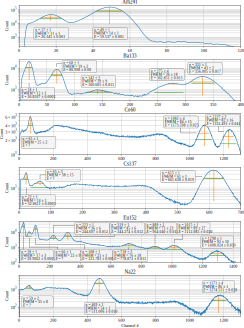
\includegraphics[width=\textwidth]{../figures/all_spectra_annotated.pdf}}
	\cprotect\caption{%
		Gamma ray spectra of the six radioisotopes tested.
		Each peak is annotated with the channel number $n$ of its centre,
		its full width at half maximum and the accepted value $E$ for its
		energy in keV (derived from \cite{heath} for gamma rays and
		\cite{shirley_1978} for X-rays).
		Orange vertical and horizontal lines extend from base to top and
		across each peak at the half-maximum height, as determined by the
		$\verb|scipy.signal.find_peaks|$ routine. Green horizontal lines
		span the peaks at half-maximum height, as determined by Lorentzian
		curve fitting.
	} 
	\label{fig:spectra}
\end{figure*}

\subsection{The spectra and their features}
Figure \ref{fig:spectra} shows the six spectra that were obtained. It
is reassuring that they are qualitatively similar to published spectra
from similar NaI(Tl) detectors (e.g., \cite{gammaspectacular}).
We were able to match the peaks to their corresponding gamma ray energies
by comparing the measured spectra and peak locations to those given by
\cite{heath} (for gamma rays) and \cite{shirley_1978} (for X-rays).
We will now examine each spectrum in detail, explaining the features
that are present. The explanations are partly drawn from the gamma spectrum
database of \cite{gammaspectacular}, the radioactive source list of
\cite{ld_didactic} and the decay schemes of \cite{shirley_1978}.

\subsubsection{Americium-241}
$^{241}$Am undergoes alpha decay to $^{237}$Np. 85\% of the product
nuclei initially exist in an excited state and then fall into the
ground state, emitting a $\SI{59.537}{\kilo\electronvolt}$ gamma photon.
This manifests as a peak near channel 50 in our spectrum. The excited nucleus
may also fall to the first excited state instead of the ground state,
emitting a $\SI{26.345}{\kilo\electronvolt}$ gamma photon; this is the source
of the peak at channel 17. Almost no signal is seen in the remainder of the
spectrum.

\subsubsection{Barium-133}
$^{133}$Ba decays via electron capture to $^{133}$Cs, whose nuclei may
initially exist in a number of excited states. The decay of these excited
states gives rise to the four highest-energy peaks in the spectrum. The
lowest-energy peak corresponds not to a gamma ray, but a characteristic
X-ray of Cs. The X-ray is produced by \emph{internal conversion}, where
the excited nucleus transfers its energy to one of its inner-shell electrons,
ejecting it from the atom instead of producing a gamma ray. A remaining
electron fills the inner-shell vacancy, emitting the X-ray photon.

\subsubsection{Cobalt-60}
$^{60}$Co undergoes beta decay to excited states of $^{60}$Ni, producing
the two photopeaks observed at the right end of the spectrum. Compton
scattering of these gamma photons in the detector produces a long
Compton continuum that spans several hundred channels, terminating at
the Compton edge near channel 900. At the left end of the continuum
(near channel 200), a wide, skewed peak is observed. This is a
\emph{backscatter} peak, created by gamma rays that undergo Compton
scattering in the lead shielding surrounding the detector and are
redirected into the detector with lower energies. Finally, the narrow
leftmost peak corresponds to a characteristic X-ray of lead; the high-energy
$^{60}$Co gamma rays eject inner-shell electrons in the detector's lead
shielding via the photoelectric effect and remaining electrons fill the
vacancy, emitting X-ray photons.

\subsubsection{Caesium-137}
$^{137}$Cs undergoes beta decay to $^{137}$Ba, 95\% of whose nuclei initially
exist in an excited state that decays, emitting a 
$\SI{661.638}{\kilo\electronvolt}$ gamma photon and producing the single
photopeak at the right end of the spectrum. The corresponding Compton continuum
and backscatter peak are seen in the middle of the spectrum, with
characteristic X-rays of barium (produced by internal conversion as previously
explained) and the lead housing at the low-energy end.

\subsubsection{Europium-152}
$^{152}$Eu decays via electron capture and positron emission to $^{152}$Sm,
which has many possible excited states. This produces seven visible gamma ray
peaks in the spectrum. Characteristic X-rays of samarium
(from internal conversion) and the lead housing are also observed.

\subsubsection{Sodium-22}
$^{22}$Na decays via electron capture and positron emission to $^{22}$Ne,
primarily into an excited state that emits a
$\SI{1274.511}{\kilo\electronvolt}$ gamma photon when it transitions to
the ground state. This produces the rightmost photopeak and Compton
continuum in the spectrum. Additionally, the positrons produced directly
by the decay of $^{22}$Na annihilate with electrons in the surrounding
material, each pair emitting two $\SI{511.005}{\kilo\electronvolt}$
gamma photons in opposite directions. This gives rise to the photopeak
near channel 470 and the corresponding Compton continuum. Characteristic
X-rays of the lead housing are observed.

\subsection{Spectrometer calibration}\label{sec:calibration}
It was mentioned in \autoref{sec:intro} that
the energy deposited into the detector should be proportional to
the amplitude of the voltage pulse sent to the multi-channel analyser
(and thus to the channel number assigned to the pulse). We now seek to
calibrate the spectrometer:
determine the constant of proportionality and use it to formulate a
relationship between channel number and energy. This step is essential
in every application of gamma ray spectrometry; the spectra are useless
without corresponding energy scales.

Our approach is to choose nine well-resolved peaks that (roughly) evenly
span the observed energy range and have good Lorentzian fits
(1408, 1275, 779, 662, 511, 344, 245, 122 and 59.5 $\si{\kilo\electronvolt}$)
to generate the calibration parameters, and use the remaining peaks to
assess the accuracy of the calibration by comparing their accepted energies
to the energies implied by the calibration parameters.

The measured centres of the peaks and uncertainties (obtained according to the
method in \autoref{sec:methods}) and corresponding accepted energies
and uncertainties (from \cite{heath}) were collated. A linear orthogonal
distance regression of energy against peak centre was performed, yielding
the relationship
\begin{equation}
	E = [(1.080 \pm 0.003) n + (3.3 \pm 1.9)] \si{\kilo\electronvolt}
	\label{eqn:calibration}
\end{equation}
where $n$ is the channel number.
Figure \ref{fig:calibration} reveals that energy is indeed a linear function
of channel number; the coefficient of determination of the fit is
$R^2 = 1 - 5.8\times10^{-5}$ and the residuals are on the order of 1\%.

\begin{figure}[ht]
	\includegraphics[width=\linewidth]{../figures/calibration.pdf}
	\caption{
		Top: plot of peak locations against accepted energy values,
		with linear ODR fit in orange. Uncertainties are too small to be
		displayed.
		Bottom: residuals of the fit in the top plot,
		corresponding to the error between the energy predicted from
		the experimental calibration and the accepted energy value.
	}
	\label{fig:calibration}
\end{figure}

Estimates for the remaining peak energies, generated using
\ref{eqn:calibration}, are displayed in Table \ref{tab:peaks}.
Seven out of sixteen predictions were consistent with the accepted values
given the prediction uncertainty, with an average error (predicted minus
accepted) of $-1.4\sigma$. The inconsistency of some of the predictions could
be due to underestimation of the uncertainty in the central channel of
particularly skewed or noisy peaks, the superposition of the peaks upon
other spectral features (or other unresolved peaks) or misidentification of
the accepted energies
(though this is unlikely). The fact that almost all the energies
were under-predicted suggests that the set of nine chosen calibration peaks
may not have been representative of the remaining peaks. This hypothesis
is supported by the fact that most of the inconsistent peaks have energies
below $\SI{100}{\kilo\electronvolt}$ and lie at the extreme lower end of
the calibration set. Future work should test the dependence of the errors
on the choice of calibration set.

\begin{table}[ht]
    \centering \scriptsize
    \csvreader[
    tabular = |c|c|c|c|,
    table head = {
    	\hline
    	\thead{\textbf{Isotope}}
    	& \thead{\textbf{Accepted}\\\textbf{energy}\\\textbf{(keV)}}
    	& \thead{\textbf{Predicted}\\\textbf{energy}\\\textbf{(keV)}}
    	& \thead{\textbf{Error}\\\textbf{(predicted}\\\textbf{minus}\\\textbf{accepted)}}
    	\\\hline\hline
    },
    late after line = \\\hline,
    ]{../figures/peak_table.csv}{}{%
    \csvcoli
    &
    \sisetup{round-mode=places, round-precision=3}
    $\num{\csvcolii} \pm \num{\csvcoliii}$
    &
    \sisetup{round-mode=places, round-precision=1}
    \ifthenelse{\equal{\csvcoliv}{}}{---}%
    	{$\num{\csvcoliv} \pm \num{\csvcolv}$}
    &
    \sisetup{round-mode=places, round-precision=1}
    \ifthenelse{\equal{\csvcoliv}{}}{---}%
    	{$\num{\csvcolvi} \sigma$}
    }%
    \cprotect\caption{%
    	Accepted values for the energies of the peaks in Figure
    	\ref{fig:spectra}, the corresponding predictions using
    	the calibration equation (\ref{eqn:calibration}) and the errors
    	as fractions of the prediction uncertainties.
    	Of course, the energies of the peaks that were used to generate
    	the calibration cannot be predicted using the same calibration,
    	and are left blank.
    }
    \label{tab:peaks}
\end{table}

\subsection{Energy resolution and intrinsic width}\label{sec:resolution}
It is evident from Figure \ref{fig:spectra} that the limited resolution of
the spectrometer has an impact on the results. For example, the
$\SI{302.851}{\kilo\electronvolt}$ and $\SI{356.005}{\kilo\electronvolt}$
peaks of $^{133}$Ba are barely resolved, and the
$\SI{39.9062}{\kilo\electronvolt}$ peak of $^{152}$Eu appears to be the
superposition of two unresolved peaks.

We will now quantitatively analyse the spectrometer's resolving power.
(\ref{eqn:resolution}) suggests that a plot of $(\Delta E/E)^2$ against
$1/E$ should yield a linear relationship with slope $B$ and intercept
$W_I^2$. Figure \ref{fig:resolution}, using the FWHM data shown in 
Figure \ref{fig:spectra} and the accepted energies
in Table \ref{tab:peaks}, does indeed support this hypothesis.
While there are two notable outliers, it is reassuring that the uncertainties
we have derived for $(\Delta E/E)^2$ generally overlap with the regression
line; this indicates that our derivation was reasonable. The magnitude
of the uncertainty results from the ambiguity of the FWHM for asymmetric
peaks, which we will discuss in more detail in \autoref{sec:discussion}.

An ordinary least squares%
\footnote{The uncertainties in the accepted energies $E$ are negligible
compared to the uncertainties in the FWHMs $\Delta E$, justifying the use
of ordinary least squares instead of orthogonal distance regression.}
regression of $(\Delta E/E)^2$ against
$1/E$ yields an intrinsic width $W_I = 0.035 \pm 0.004$ for our detector.
The fact that this is clearly nonzero is consistent with
the findings of \cite{zerby_1961}, who observed an ``intrinsic line
broadening'' in Monte Carlo simulations of NaI(Tl) gamma ray spectrometers.

\begin{figure}[ht]
	\includegraphics[width=\linewidth]{../figures/resolution.pdf}
	\caption{
		Plot of $(\Delta E/E)^2$ against $1/E$, with a linear fit yielding \
		an intrinsic width $W_I = 0.035 \pm 0.004$.
		A log-log scale is used instead of a linear one so that the
		datapoints in the lower left corner are clearly distinguishable.
		The uncertainty in 
		$1/E$ is negligible compared to the uncertainty in $(\Delta E/E)^2$.
	}
	\label{fig:resolution}
\end{figure}

\subsection{Full energy peak efficiency}
The detector's full energy peak efficiency (hereafter FEPE)
is the fraction of gamma photons
produced at a given energy by the source that are counted in the spectrum's
corresponding full energy peak. Eight full energy peaks
(as in \autoref{sec:calibration}, well-resolved peaks that (roughly) evenly
span the observed energy range) were chosen for analysis: 1408,
1275, 662, 511, 344, 245, 122 and 59.5 $\si{\kilo\electronvolt}$.

The net count rates for the peaks were determined by summing the counts
in each peak's constituent channels, subtracting the contribution of the counts
below the baseline level of the peak and dividing by the count time.
The horizontal extent of each peak was determined subjectively rather than
programmatically to ensure that the choices were reasonable. This naturally
introduced undesirable uncertainties in the count sums; their magnitude
was estimated by re-calculating the sums after extending all the windows by
10\% (a value chosen arbitrarily but based on the expected level of
uncertainty) in both directions, and then after contracting all the windows by the
same amount. The uncertainty was taken to be half of the difference between
the extended and contracted values. 

The rate of corresponding gamma photon emission for each peak was determined
by multiplying the total activity of the appropriate radioisotope sample
(computed from the activity of the sample on its manufacturing date
and the length of time since manufacturing)
by the known relative gamma ray intensity at that energy (obtained from
\cite{notes}). Dividing the net count rate by the rate of gamma photon
emission yielded the FEPE, shown as a function
of energy in Figure \ref{fig:efficiency}.
As a first approximation, we neglect uncertainties in peak height
and sample activity compared to the aforementioned uncertainties
due to subjective choice of peak extent.

\begin{figure}[ht]
	\centering
	\includegraphics[width=\linewidth]{../figures/efficiency.pdf}
	\caption{
		Plot of net FEPE against
		peak energy. The uncertainty in energy is negligible.
	}
	\label{fig:efficiency}
\end{figure}

We observe a FEPE that is approximately constant at energies below
$\SI{2e2}{\kilo\electronvolt}$ but decreases roughly exponentially
with increasing energy beyond this point.
In fact, \cite{theoretical_fepe} devised a theoretical scheme for
predicting the FEPE of a NaI(Tl) gamma spectrometer.
While the details of the scheme and its derivation are highly non-trivial and
entirely beyond the scope of this paper, we may at least qualitatively
compare our results to theirs. They presented calculations
for a wide range of detector geometries and positions; in Figure
\ref{theoretical_fepe}, we reproduce their Figure 6, which concerns
the FEPE as a function of energy for
one particular detector and position (the others are qualitatively similar,
having the same decline in efficiency). Remarkably, this bears
an extremely close resemblance to our Figure \ref{fig:efficiency};
even the numerical values are similar. This is strong evidence that
our approach to measuring FEPE is valid and reasonably accurate.
Future work could attempt a more quantitative comparison by
applying the theoretical scheme to our detector.

\begin{figure}[ht]
	\centering
	\includegraphics[width=\linewidth]{../figures/theoretical_fepe.pdf}
	\cprotect\caption{%
		Reproduction of Figure 6 in the paper by \cite{theoretical_fepe},
		showing
		the calculated theoretical efficiencies for two radioactive sources
		(``V1'' and ``V2'') as solid lines. These are consistent with
		measured values (red dots and pink squares). Note the extremely close
		resemblance to Figure \ref{fig:efficiency}.
	}
	\label{theoretical_fepe}
\end{figure}

\begin{comment}
\subsection{Electron mass}
(\ref{eqn:compton_edge}) may be inverted to yield
\begin{equation*}
	m_e = \frac{2E}{c^2} \left( \frac{E}{E_c} - 1 \right),
\end{equation*}
which can be used to estimate the electron mass, given $E$ and $E_c$.
To illustrate this, we estimate $E_c = \SI{975 \pm 50}{\kilo\electronvolt}$
for the $E = \SI{1173.208}{\kilo\electronvolt}$ gamma ray of $^{60}$Co by
close inspection of Figure \ref{fig:spectra} and channel-to-energy conversion
using (\ref{eqn:calibration}). This gives
$m_e = \SI[per-mode=symbol]{0.48 \pm 0.15}{\mega\electronvolt\per\clight\tothe{2}}$,
consistent with the accepted value
$\SI[per-mode=symbol]{0.5110}{\mega\electronvolt\per\clight\tothe{2}}$
\citep[p. 47]{codata}.
The magnitude of the uncertainty is, admittedly, very large due to the
uncertainty in the position of the Compton edge, which appears as a gradual
decline in the spectrum rather than a sharp drop.
\end{comment}

\section{Discussion} \label{sec:discussion}
We shall now discuss the factors that influenced the quality of our results
and measures that may be taken in future work to mitigate them.

\subsection{Determining peak location and FWHM}
\autoref{sec:methods} alluded to difficulties in characterising the
peaks in our gamma ray spectra in justifying the final approach used;
we now extend this discussion. The method of Lorentzian curve fitting has
several disadvantages, including
\begin{itemize}
	\item The fact that the peaks may not be Lorentzian at all,
		as evidenced by decreases in fit quality when the subsets of
		the spectra considered ``part of the peaks'' were expanded
		(reducing the validity),
	\item The superposition of the peaks upon other spectral features
		(such as other peaks and their Compton continua),
		skewing them from the assumed Lorentzian shape, which must be
		symmetrical for an accurate fit,
	\item Ambiguity in the base levels of the peaks
		(the parameter $b$ in (\ref{lorentzian}), which was determined
		by the fitting routine with the sole aim of reducing mean
		squared error, neglecting physical considerations (before the
		addition of constraints, the calculated base level was often negative),
	\item The consequent ambiguity in the FWHM due to ambiguity in the
		base level, and
	\item Impossibly small reported uncertainties in the fit parameters
		(much less than one channel in peak location and FWHM),
		which were simply incompatible with the observed fit quality.
\end{itemize}
After observing the above limitations, the $\verb|scipy.signal.find_peaks|$
routine, whose operation is explained in \autoref{sec:methods}, was chosen
because it is able to characterise the peaks while making far weaker
assumptions about their shape. In particular, the routine's approach to
determining the baseline level of a peak is, physically, much more reasonable.
The reported FWHM value also corresponds to the literal width of the
peak at some height, rather than an inferred width from a fit that may
deviate from the true peak shape. Nonetheless, the routine also has
its limitations, including
\begin{itemize}
	\item The fact that it simply takes the location and height of the
		highest data point as the location and height of the peak,
		and similarly for the base and FWHM measurements, increasing
		the impact of random noise compared to curve fitting (which recognises
		a distribution of data points about the fitted curve), and
	\item Its inability to natively estimate the uncertainties in
		the peak parameters, forcing an \emph{ad hoc} solution
		based partly in estimation and human judgement rather than
		mathematics.
\end{itemize}
We have used the discrepancy between the two approaches to our advantage.
The Lorentzian method usually underestimated the peaks' base levels
and overestimated their FWHMs, while the SciPy routine may have done the
opposite, overestimating the base levels by choosing the higher
of the minima to the left and right of each peak. This is
evidenced by the fact that the green
horizontal Lorentzian half-maximum lines in Figure \ref{fig:spectra}
invariably lie lower than the yellow half-maximum lines from the
SciPy routine. We therefore conjectured that the true half-maximum level
should lie between these two estimates, leading us to our final values
and uncertainties.

Future work should further investigate the methods of
peak characterisation used in modern-day research and evaluate their
performance.

\subsection{Resolution limits}
The limited resolving power of the detector, as investigated in
\autoref{sec:resolution}, is an inherent feature of the family of
scintillation detectors, of which our NaI(Tl) detector is a member.
Another approach to gamma ray detection uses semiconductors,
whose electrons may be excited from the valence band to the conduction
band by incoming gamma photons. The arrival of gamma photons thus
increases the conductivity of the semiconductor, which may be measured
electrically. Semiconductor detectors have far better resolving power
than scintillators, but must be kept at cryogenic temperatures,
making them infeasible for future work in the teaching laboratory.
Comparison of our spectra to those of \cite{heath}, who used silicon
and germanium semiconductor detectors, clearly shows that we were only
able to observe a small subset of the many gamma energies present.

\section{Conclusion} \label{sec:conclusion}
We have successfully acquired the gamma ray spectra of six radioisotope
samples using a NaI(Tl) scintillation detector and shown that the
theory governing the
fundamental processes occurring in the source and detector justifies
their appearance. 

We calibrated the spectrometer and assessed
the accuracy of energies predicted using the calibration, finding that
although some of the predictions were consistent with expectations,
others were not due to other uncertainty sources, the superposition of peaks
on other spectral features or misidentification of peaks with accepted
energy values.

We then calculated the detector's resolution, which improved with
increasing gamma ray energy, and calculated its intrinsic width, the
fundamental limit on its resolution. The existence of this fundamental limit
is consistent with the behaviour expected for NaI(Tl) detectors based
on computer models.

Finally, we calculated the full energy peak efficiency of the detector as
a function of energy and demonstrated a remarkable agreement between our
results and theoretical values.

In summary, we have demonstrated the utility of scintillation-based
gamma ray spectrometry, as well as its limitations. Our findings will be
useful in the design of future investigations into gamma spectrometry.

\clearpage
\acknowledgments
The author gratefully acknowledges the assistance of the UNSW School of Physics,
which provided the facilities and equipment for this work, the staff
in the UNSW Higher Year Physics Laboratory, who provided guidance during
the experiment, and his laboratory partner Oscar Prien, with whom he had
enlightening discussions.

\datastatement
The raw data and Python code used to produce the results in this report
are available as supplementary material
at \url{https://github.com/tschanzer}.
They are also available from the author upon request.

\bibliographystyle{ametsocV6}
\bibliography{references}


\end{document}